\documentclass[../bericht.tex]{subfiles}

\begin{document}

  \chapter{Versuchsdurchführung und -auswertung}

    Im folgenden Kapitel werden die einzelnen Schritte der Versuchsdurchführung und die jeweilige Analyse parallel beschrieben.


    \section{Vorbereitende Messungen}


      \subsection{Dunkelspektrum}

        Das Spektrometer zeichnet auch ohne Einschalten des Lasers bereits Signale auf. Dies liegt in diesem Falle nicht am Streulicht anderer Lichtquellen im Raum, wie durch das Ausbleiben von Veränderungen im Signal während dem Ein- und Ausschalten von prominenten Lichtquellen wie der Deckenleucchte leicht bewiesen werden kann. Vielmehr kommt es in der Ladungsträgerzone der Dioden zu spontanen Elektron-Loch-Paar-Bildungen, welche als Photonen registriert werden. Mit dem zu Auswertung verwendeten Programm \textit{???} wird deshalb bei jeder Änderung der Integrationszeit während der Versuche ein neues Dunkelspektrum aufgezeichnet, das heißt mit geblocktem Laserstrahl einmal die Integrationszeit durchlaufen. Dieses Dunkelspektrum subtrahiert das Programm dann von jedem weiteren aufgenommenen Spektrum automatisch, sodass der Untergrund weitgehen bereinigt ist.


      \subsection{Kalibrierung des Spektrometers}
      \label{subsec:kalibrierung}

        \begin{figure}[tb]
          \centering
          \tikzsetnextfilename{hg_he_spektren}
          \begin{tikzpicture}
            \begin{axis}[
              /tikz/line join=bevel,
              width=0.8*\textwidth,
              height=0.5*\textwidth,
              grid,
              legend style={at={(1,1)}, legend columns=1, anchor=north east},
              every axis plot,
              xmin = 490, xmax = 680,
              %ymin = \Pmin, ymax = \Pmax,
              xlabel = {Wellenlänge $\lambda$ in $\si{\nano\meter}$},
              ylabel = {Zählrate $n$},
              /pgf/number format/use comma,
              /pgf/number format/1000 sep={},
              ]
              % Add plots
              \addplot[color=red!30, only marks, line width = 0.5pt, mark options={scale=0.2}] table [x=lambda,y=n]{data/hg_spektrum_fit.txt};
              \addlegendentry{Hg data points}
              \addplot[color=red, line width = 0.5pt] table [x=lambda,y=fit]{data/hg_spektrum_fit.txt};
              \addlegendentry{Hg fit}
              \addplot[color=blue!30, only marks, line width = 0.5pt, mark options={scale=0.2}] table [x=lambda,y=n]{data/he_spektrum_fit.txt};
              \addlegendentry{He data points}
              \addplot[color=blue, line width = 0.5pt] table [x=lambda,y=fit]{data/he_spektrum_fit.txt};
              \addlegendentry{He fit}
            \end{axis}
          \end{tikzpicture}
          \caption{}
          \label{fig:hg-he-spektren}
        \end{figure}

        Um die Wellenlängen-, bzw. Frequenz-Kalibrierung des Spektrometers zu prüfen und gegebenenfalls zu korrigieren werden zwei Messungen mit in der Literatur hinreichend präzise charakterisierten Lichtquellen durchgeführt. Die aufgezeichneten Spektren einer Quecksilberdampflampe und einer Heliumlampe sind in \cref{fig:hg-he-spektren} abgebildet.  Die charakteristischen Linien treten hier verbreitert in Erscheinung. Es liegen die Dopplerverbreiterung, die Verbreiterung durch die natürliche Linienbreite, sowie die linear mit dem Dampfdruck ansteigende Druckverbreiterung vor. Prominent ist hierbei die Dopplerverbreiterung. Wegen der gaussförmigen Maxwell-Boltzmann-Verteilung der Geschwindigkeit der Gasatome können die verbreiterten Linien zu Bestimmung der Position der Maxima mit Gaussfits approximiert werden. Diese sind ebenfalls in \cref{fig:hg-he-spektren} aufgetragen. Die so gemessenen Linienpositionen mitsamt der aus \cite{NIST_ASD} entnommenen Literaturwerte sind in \cref{tbl:charakteristische-linien} aufgeführt. Die bei den experimentellen Werten angegebenen Unsicherheiten sind lediglich die Fehler der Fitparameter. Diese sind natürlich deutlich zu klein, wenn die Unsicherheiten aufgrund der  und Messunsicherheiten der verwendeten Geräte selbst noch respektiert werden. Dementsprechend stimmen die gemessenen Wellenlängen der charakteristischen Linien der Lichtquellen, vor Allem unter berücksichtigung der Breite der Guassglocken, hinreichend präzise mit den Literaturwerten überein, um keine weiteren Korrekturen vornehmen zu müssen.
        \medskip

        \begin{table}[tb]
        \caption[Experimentelle und Literaturwerte (\cite{NIST_ASD}) der charakteristischen Linien der Quecksilberdampflampe und der Heliumlampe.]{Experimentelle und Literaturwerte (\cite{NIST_ASD}) der charakteristischen Linien der Quecksilberdampflampe und der Heliumlampe zum Prüfen der Kalibrierung des Spektrometers. Für die weitere Interprätation siehe \cref{subsec:kalibrierung}}
        \label{tbl:charakteristische-linien}
        \selectfontsize{10pt}
        \begin{tabu} {X[r]X[r]X[r]X[r]X[r]X[r]X[r]}
          \unitoprule \\
          &\multicolumn3{c}{\textbf{Hg}}  &\multicolumn3{c}{\textbf{He}}  \\
          \unimidrule \\
          $\lambda_\mathrm{exp}$ $[\si{\nano\meter}]$ &546,075  &576,961  &579,067  &501,569  &587,562  &667.815 \\
          $\lambda_\mathrm{lit}$ $[\si{\nano\meter}]$ &546,237(1)  &577,128(2)  &579,241(3) &501,572(41)  &587,752(01)  &668,274(09) \\
          \unitoprule \\
        \end{tabu}
        \end{table}

        Natürlich ist der Nd:YAG-Laser. Ein Spektrum ohne Streuer wurde aber nicht aufgezeichnet und so soll hier vorab darauf verwiesen werden, dass das Maximum der Rayleigh-Streuung bezüglich der Raman-Verschiebung in allen späteren Messungen auf $\sim\SI{0}{\per\centi\meter}$ liegt und damit aufgrund der Einstellung des verwendeten Analyseprogramms bei $\SI{532}{\nano\meter}$. Dies bestätigt wiederum die zuvor gemachte Behaupttung, dass das Spektrometer hinreichend präzise für dieses Experiment kalibriert ist.


      \subsection{Linearität des Spektrometers}
      \label{subsec:linearitaet}

        \begin{figure}[tb]
          \tikzsetnextfilename{linearity}
          \begin{tikzpicture}
            \begin{axis}[
              /tikz/line join=bevel,
              width=0.8*\textwidth,
              height=0.5*\textwidth,
              grid,
              legend style={at={(1,1)}, legend columns=1, anchor=north east},
              every axis plot,
              xmin = 666, xmax = 671,
              %ymin = \Pmin, ymax = \Pmax,
              xlabel = {Wellenlänge $\lambda$ in $\si{\nano\meter}$},
              ylabel = {Zählrate $n$},
              ]
              % Add plots
              \addplot[color=red,  line width = 0.5pt] table [x=lambda,y=n]{data/he_50.txt};
              \addlegendentry{$\SI{50}{\milli\second}$}
              \addplot[color=blue,  line width = 0.5pt] table [x=lambda,y=n]{data/he_100.txt};
              \addlegendentry{$\SI{100}{\milli\second}$}
              \addplot[color=green,  line width = 0.5pt] table [x=lambda,y=n]{data/he_200.txt};
              \addlegendentry{$\SI{200}{\milli\second}$}
              \addplot[color=orange,  line width = 0.5pt] table [x=lambda,y=n]{data/he_400.txt};
              \addlegendentry{$\SI{400}{\milli\second}$}
              \addplot[color=purple,  line width = 0.5pt] table [x=lambda,y=n]{data/he_800.txt};
              \addlegendentry{$\SI{800}{\milli\second}$}
              \addplot[color=brown,  line width = 0.5pt] table [x=lambda,y=n]{data/he_2000.txt};
              \addlegendentry{$\SI{2000}{\milli\second}$}
              \addplot[color=violet,  line width = 0.5pt] table [x=lambda,y=n]{data/he_3000.txt};
              \addlegendentry{$\SI{3000}{\milli\second}$}
              \addplot[color=cyan,  line width = 0.5pt] table [x=lambda,y=n]{data/he_4000.txt};
              \addlegendentry{$\SI{4000}{\milli\second}$}
            \end{axis}
          \end{tikzpicture}
          \caption[Spektren der $\sim\SI{668}{\nano\meter}$-Linie der Heliumlampe bei verschiedenen Integrationszeiten zur Prüfung der Linearität des Spektrometers.]{Spektren der $\sim\SI{668}{\nano\meter}$-Linie der Heliumlampe bei verschiedenen Integrationszeiten zur Prüfung der Linearität des Spektrometers. Für weitere Ausführungen siehe \cref{subsec:linearitaet}}
          \label{fig:linearity}
        \end{figure}

        Das Spektrometer zählt unter Verwendung von Dioden die, nach Wellenlänge sortierten, einfallenden Photon. Bei zeitlich konstanter Lichtquelle sollte also die Zahl $n$ der registrierten Photonen pro wellenlänge linear zunehmen. Um dies zu überprüfen sind in \cref{fig:linearity} die Spektren der Heliumlampe für verschiedene Integrationszeiten aufgetragen. An dieser Stelle ist zu beachten, dass das Spektrometer 16 Bit basiert ist und damit eine Zählrate von $2^{16}\approx 65000$ nicht überschreiten kann.

        Die Zählrate der lokalen $\sim\SI{668}{\nano\meter}$-Maxima der Spektren werden mithilfe von \textit{Python} aus den Rohdaten extrahiert, deses Mal ohne die Verwendung eines Fits. Aufgetragen über den Integrationszeiten ergibt sich, wie erwartet, ein linearer Zusammenhang, wie in \cref{fig:linearitaet} abgebildet ist. Die Gleichung der linearen Regression durch den Ursprung ist
        \begin{equation}
          n(t_\mathrm{int})=\SI{8,386(1)}{\per\milli\second} \cdot t_\mathrm{int}.
          \label{eq:linear-fit}
        \end{equation}
        Messpunkte und Regression liegen übereinander, was die Linearität des Spektrometers unterhalb der Sättigungsgrenze bestätigt.

        \begin{figure}
          \centering
          \tikzsetnextfilename{linear_fit}
          \begin{tikzpicture}
            \begin{axis}[
              /tikz/line join=bevel,
              width=0.8*\textwidth,
              height=0.5*\textwidth,
              grid,
              legend style={at={(1,0)}, legend columns=1, anchor=south east},
              every axis plot,
              xmin = 0, xmax = 5,
              ymin = 0, ymax = 35000,
              xlabel = {Integrationszeit $t_\mathrm{int}$ in $\si{\second}$},
              ylabel = {Zählrate $n$},
              /pgf/number format/use comma,
              /pgf/number format/1000 sep={},
              ]
              % Add plots
            	\addplot[color=red, only marks] coordinates {
            		(0.05,382.97)
            		(0.1,827.38)
            		(0.2,1605.61)
            		(0.4,3205.07)
            		(0.8,6782.87)
            		(2,16725.76)
            		(4,33572.35)
            	};
              \addlegendentry{Messpunkte}
              \addplot[color=blue, line width=1pt] gnuplot{8386.15286*x};
              \addlegendentry{Lineare Regression}
            \end{axis}
          \end{tikzpicture}
          \caption[Messpunkte der $\sim\SI{668}{\nano\meter}$-Maxima der Heliumlampen-Spektren bei verschiedenen Integrationszeiten (vgl. \cref{fig:linearity}) und lineare Regression.]{Messpunkte der $\sim\SI{668}{\nano\meter}$-Maxima der Heliumlampen-Spektren bei verschiedenen Integrationszeiten und lineare Regression gemäß \cref{eq:linear-fit}.}
          \label{fig:linearitaet}
        \end{figure}


      \subsection{Kerbfilter}
      \label{subsec:kerbfilter}

        Um die Breite und Position des Wellenlängenbereichs, welchen der Kerbfilter blockt, zu messen, wird eine Handytaschenlampe als breitbandige Lichtquelle genutzt. \Cref{fig:kerbfilter-spektren} zeigt Spektren des Handys mit und ohne Kerbfilte im Strahlengang. Dabei ist der Kerbfilter in der Nullposition $\varphi=0$ um $\ang{90}$ gegen den Strahlengang gedreht. Die weiteren Drehwinkel sind als Drehung gegen die Nullposition gemessen und aufgrund der Messung mittels Millimeterpapier stark Messunsicherheitsbehaftet ($\delta \varphi=\pm \ang{1}$). Durch die Drehung des Kerbfilters (Dünnschichtfilter) vergrößert sich die vom Licht zu transmittierende Schichtdicke und damit verschieben sich die geblockten Wellenlängen zu kleineren Werten. Hierbei ist die Verschiebung nach einfacher Geometrie unabhängig von der Drehrichtung. Die Breite des geblockten Wellenlängenintervalls wird in den folgenden Aalysen eine Rolle spielen.

        \begin{figure}[tb]
          \centering
          \tikzsetnextfilename{kerbfilter}
          \begin{tikzpicture}
            \begin{axis}[
              /tikz/line join=bevel,
              width=0.8*\textwidth,
              height=0.5*\textwidth,
              grid,
              legend style={at={(1,1)}, legend columns=1, anchor=north east},
              every axis plot,
              xmin = 480, xmax = 660,
              %ymin = \Pmin, ymax = \Pmax,
              xlabel = {Wellenlänge $\lambda$ in $\si{\nano\meter}$},
              ylabel = {Zählrate $n$},
              /pgf/number format/use comma,
              /pgf/number format/1000 sep={},
              ]
              % Add plots
              \addplot[color=red,  line width = 0.5pt] table [x=lambda,y=n]{data/handy_ohne_kerb.txt};
              \addlegendentry{Ohne Kerbfilter}
              \addplot[color=blue,  line width = 0.5pt] table [x=lambda,y=n]{data/handy_mit_kerb.txt};
              \addlegendentry{$\varphi=\ang{0}$}
              \addplot[color=green,  line width = 0.5pt] table [x=lambda,y=n]{data/handy_mit_kerb_5_grad.txt};
              \addlegendentry{$\varphi=\ang{5}$}
              \addplot[color=orange,  line width = 0.5pt] table [x=lambda,y=n]{data/handy_mit_kerb_10_grad.txt};
              \addlegendentry{$\varphi=\ang{10}$}
              \addplot[color=magenta,  line width = 0.5pt] table [x=lambda,y=n]{data/handy_mit_kerb_15_grad.txt};
              \addlegendentry{$\varphi=\ang{15}$}
            \end{axis}
          \end{tikzpicture}
          \caption[Spektren einer Handytaschenlampe mit um den Winkel $\varphi$ gedrehten Winkel und ohne Kerbfilter.]{Spektren einer Handytaschenlampe mit um den Winkel $\varphi$ gedrehten Winkel und ohne Kerbfilter. Relevant ist die Verschiebung des durch den Kerbfilter entstehende Minimum des Transmissionsspektrum und dessen Verschiebung zu kürzeren Wellenlängen mit größer werdendem $\varphi$.}
          \label{fig:kerbfilter-spektren}
        \end{figure}




    \section{Abschätzung der zu erwartenden Raman-Verschiebungen}
    \label{subsec:harm-oszi-absch}

      Zunächst soll anhand eines einfachen harmonischen Oszillator Modells zweier Atome die zu erwartenden Raman-Verschiebungen in Abhängikeit der beteiligten Elemente abgeschätzt werden (vgl. \cref{subsec:harm-oszi-absch}).

      Als Basis der theoretischen Erwartung dient die Streckschwingung einer H-H-Bindung, deren Raman-Verschiebung nach \cite{herzberg} bei
      \begin{equation*}
        \nu_\mathrm{H-H}=\frac{1}{\lambda_0}-\frac{1}{\lambda}=\SI{4160}{\per\centi\meter},
      \end{equation*}
      mit der Wellenlänge des eingestrahlten Lichts $\lambda_0$ und der Wellenlänge der Raman-Maxima $\lambda$, liegt. Mit \cref{eq:omega} ergibt sich die Bindungsenergie des harmonischen Oszillators zu
      \begin{equation*}
        E=\frac{\mu}{2}\omega^2x_0^2=\frac{\mu}{2}\left[ 2\pi c \underbrace{\left( \frac{1}{\lambda_0} - \frac{1}{\lambda} \right)}_{=\nu} \right]^2x_0^2
      \end{equation*}
      wobei $\mu$ wie zuvor die reduzierte Masse ist und $c$ die Lichtgeschwindigkeit. Unter der Annahme, dass die Bindungsenergie für andere Atome gleich groß ist, folgt der Zusammenhang
      \begin{equation}
        \nu_\mathrm{Atom1-Atom2}=\sqrt{\frac{\mu_\mathrm{H-H}}{\mu_\mathrm{Atom-1-Atom2}}}\cdot \nu_\mathrm{H-H}.
        \label{eq:theo-raman-versch}
      \end{equation}
      Damit ergeben sich die in Tabelle \cref{tbl:theo-raman-versch} aufgeführten Raman-Verschiebungen für ausgewählte, in folgender Analyse relevanten, Atombindungen. Zur Berechnung wurden die in \cite{NIST_MASS} aufgeführten Atommassen verwendet.

      \begin{table}[tb]
      \caption[Theoretische Raman-Verschiebung verschiedener Atomkombinationen auf Grundlage des harmonischen Oszillator Modells unter Vorraussetzung der H-H-Bindungsenergie.]{Theoretische Raman-Verschiebung verschiedener Atomkombinationen auf Grundlage des harmonischen Oszillator Modells unter Vorraussetzung der H-H-Bindungsenergie. Die Werte wurden mit der Raman-Verschiebung einer H-H-Bindung $\nu_\mathrm{H-H}=\SI{4160}{\per\centi\meter}$ \cite{herzberg} und den in \cite{NIST_MASS} aufgeführten Atommassen nach \cref{eq:theo-raman-versch} berechnet.}
      \label{tbl:theo-raman-versch}
      \selectfontsize{10pt}
      \begin{tabu} {X[r]X[r]X[r]X[r]X[r]X[r]X[r]X[r]}
        \unitoprule \\
        &C-H  &C-D  &C-Cl &C-C  &O-H  &C-O  &N-O  \\
        \unimidrule \\
        $\Delta\nu$ $[\si{\nano\meter}]$ &3063 &2249 &988 &1206 &3033 &1128 &1081\\
        \unitoprule \\
      \end{tabu}
      \end{table}


    \section{Chlormethane}

      In diesem Abschnitt werde die Spektren der betrachteten Chlormethane analysiert. Ziel ist die Zuordnung der auftretenden Raman-Linien zu den  Molekülschwingungen. Weiter wird mithilfe des eingeführten harmonischen Oszillator Modells die Veränderung der Raman-Linien bei Austauschen eines, oder mehrerer Atome in einem Molekül vorherzusagen versucht.


      \subsection{Tetrachlormethan}
      \label{subsec:tetrachlor}

        \begin{figure}[tb]
          \subfloat[]{
            \tikzsetnextfilename{CCl4}
            \begin{tikzpicture}
              \begin{axis}[
                /tikz/line join=bevel,
                width=0.45*\textwidth,
                height=0.45*\textwidth,
                grid,
                legend style={at={(1,1)}, legend columns=1, anchor=north east},
                every axis plot,
                xmin = -1000, xmax = 1000,
                %ymin = \Pmin, ymax = \Pmax,
                xlabel = {Raman-Verschiebung $\Delta \nu$ in $\si{\per\centi\meter}$},
                ylabel = {Zählrate $n$},
                /pgf/number format/use comma,
                /pgf/number format/1000 sep={},
                ]
                % Add plots
                \addplot[color=red,  line width = 0.5pt] table [x=raman,y=n]{data/CCl4_pol0.txt};
                \addlegendentry{$\theta_\mathrm{pol}=\ang{0}$}
              \end{axis}
            \end{tikzpicture}
            \label{fig:ccl4}}
          \subfloat[]{
            \tikzsetnextfilename{CCl4_beide}
            \begin{tikzpicture}
              \begin{axis}[
                /tikz/line join=bevel,
                width=0.45*\textwidth,
                height=0.45*\textwidth,
                grid,
                legend style={at={(1,1)}, legend columns=1, anchor=north east},
                every axis plot,
                xmin = 0, xmax = 1600,
                %ymin = \Pmin, ymax = \Pmax,
                xlabel = {Raman-Verschiebung $\Delta \nu$ in $\si{\per\centi\meter}$},
                ylabel = {Zählrate $n$},
                /pgf/number format/use comma,
                /pgf/number format/1000 sep={},
                ]
                % Add plots
                \addplot[color=red,  line width = 0.5pt] table [x=raman,y=n]{data/CCl4_pol0.txt};
                \addlegendentry{$\theta_\mathrm{pol}=\ang{0}$}
                \addplot[color=blue,  line width = 0.5pt] table [x=raman,y=n]{data/CCl4_pol1.txt};
                \addlegendentry{$\theta_\mathrm{pol}=\ang{90}$}
              \end{axis}
            \end{tikzpicture}
            \label{fig:ccl4-beide}}
          \caption[Spektren der $\mathrm{CCl_4}$-Probe mit Polarisationsfilter in der Nullstellung und in der dazu orthogonalen Position.]{Spektren der $\mathrm{CCl_4}$-Probe mit Polarisationsfilter in der Nullstellung und in der dazu orthogonalen Position. \protect\subref{fig:ccl4} zeigt nur das Spektrum mit Polarisationsfilter in der Nullstellung für negative und positive Werte der Raman-Verschiebung. \protect\subref{fig:ccl4-beide} vergleicht lediglich den positiven Teil der Raman-Verschiebung-Achse mit Polarisationsfilter in beiden Stellungen.}
          \label{fig:ccl4}
        \end{figure}

        \Cref{fig:ccl4} zeigt das Spektrum der Tetrachlormethan-Probe ($\mathrm{CCl_4}$) mit eingesetztem Polarisationsfilter. Der Winkel $\theta_\mathrm{pol}$ gibt hierbei den Drehwinkel des Polarisationsfilter an, wobei $\theta=\ang{0}$ die Nullpolarisationsstellung bezeichnet. Bei letzter Einstellung sind alle Raman-Maxima sichtbar, polarisierte zu symmetrischen Schwingungen gehörige und depolarisierte. Weiter liegt der Kerbfilter im Strahlengang, um das prominente Maximum der Rayleigh-Streuung zu schwächen. Da der Wellenlängenbereich, welcher durch den Kerbfilter unterdrückt wird, recht breit ist (vgl. \cref{subsec:kerbfilter}), verschwinden hierdurch auch die einige der Raman-Maxima auf der linken Seite (negative Raman-Verschiebung) des Rayleigh-Maximums. Da die Stokes- und Anti-Stokes-Maxima aber symmetrisch um das Rayleigh-Maximum verteilt liegen, reicht es für die Charakterisierung der Raman-Linien eine Seite zu betrachten.
        \medskip

        \Cref{fig:ccl4-beide} zeigt nun den positiven Bereich der Raman-Verschiebung der $\mathrm{CCl_4}$-Probe mit Polarisationsfilter in der Nullstellung und der um $\ang{90}$ gedrehten Stellung. Insgesamt sind für die Nullpolarisationsstellung sechs oder sieben Raman-Maxima zu erkennen. An dieser Stelle ist noch unklar, ob das Maximum des Signals bei $\sim \SI{777}{\per\centi\meter}$ zu einem einzelnen Singulett oder zwei dicht beieinanderliegenden Linien eines Dupletts gehört.

        Nun lässt sich aufgrund der in \cref{subsec:harm-oszi-absch} berechneten theoretischen Raman-Verschiebung von $\SI{988}{\per\centi\meter}$ für eine einfache C-Cl-Bindung das Maximum bei $\sim \SI{1533}{\per\centi\meter}$ als Fundamentalschwingung ausschließen (bei allen anderen Schwingungen sind mehr Atome oder schwere Atome beteiligt). Damit verbleiben noch vier oder fünf Maxima.

        Bei Betrachtung des Spektrum mit $\theta=\ang{90}$ fällt auf, dass nur das Maximum bei $\sim\SI{451}{\per\centi\meter}$ polarisiert, die zugehörige Schwingung also symmetrisch ist, während alle anderen depolarisiert sind.

        \Cref{fig:tetraeder-schwingungen} zeigt die möglichen Schwingungen eines $\mathrm{XY_4}$-Moleküls (X, Y seien Elemente). Offensichtlich sind drei Schwingungen in der zweiten, bzw. dritte Zeile mit Drehungen und Spiegelungen an Ebenen ineinander überführbar. Das heißt die Schwingungen sind dreifach entartet. Weil auch die Schwingungen $\nu_{2j}$, $j\in\{a,b\}$, zweifach entartet ist, erwartet man insgesamt vier Fundamentalschwingungen. Die einzige symmetrische Schwingung ist die Schwingung $\nu_1$, welche somit dem fast vollständig polarisierten Maximum bei $\sim\SI{451}{\per\centi\meter}$ zugeordnet werden kann.
        \medskip

        Weiter lässt sich die Streckschwingung eines C-Cl-Paares als Superposition der $\nu_{3i}$, $i\in\{ a,b,c\}$ darstellen. Für die Streckschwingung wurde in \cref{subsec:harm-oszi-absch} eine Raman-Verschiebung von $\nu_\mathrm{C-Cl}=\SI{988}{\per\centi\meter}$ abgeschätzt. Aufgrund des für die Abschätzung verwendeten vereinfachten Modells lässt sich hiermit die Zuordnung des Maximums bei $\sim \SI{777}{\per\centi\meter}$ zur den entarteten $\nu_{3i}$ Schwingungen aus \cref{fig:tetraeder-schwingungen}, trotz der großen Abweichung von über $\SI{200}{\per\centi\meter}$, rechtfertigen. Schließlich liegt wechselwirken bei der Überlagerung der Schwingungen mehr als nur die beiden für die Streckschwingung betrachteten Atome.
        \medskip

        \begin{figure}[p]
          \centering
          \subfloat[]{
            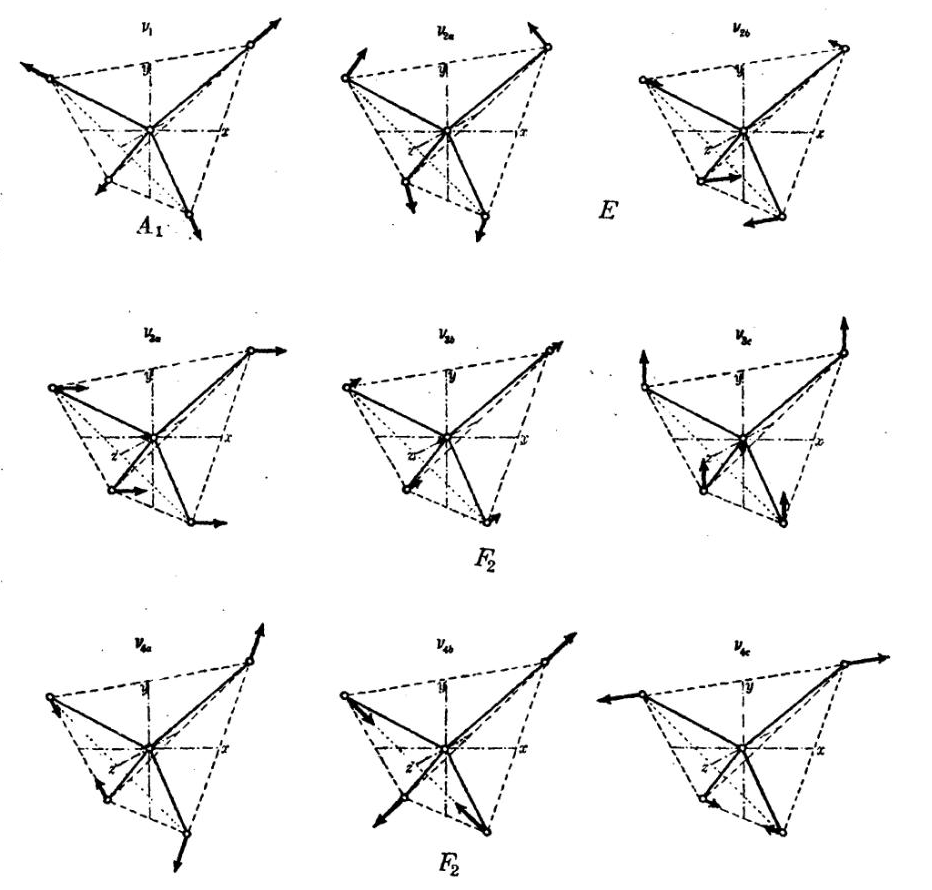
\includegraphics[width=0.8\textwidth]{figures/tetraeder.png}
            \label{fig:tetraeder-schwingungen}}  \\
          \subfloat[]{
            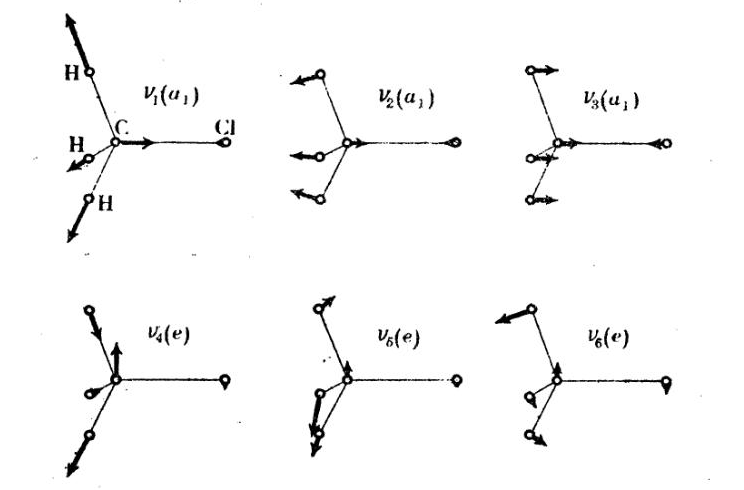
\includegraphics[width=0.8\textwidth]{figures/ch3cl.png}
            \label{fig:chcl3-schwingungen}}
          \caption[Mögliche Schwingungen eines tetraedischen Moleküls.]{Mögliche Schwingungen eines tetraedischen Moleküls. \protect\subref{fig:tetraeder-schwingungen} zeigt die Schwingungen für ein $\mathrm{XY_4}$-Molekül, \protect\subref{fig:chcl3-schwingungen} die eines $\mathrm{CH_3Cl}$-Moleküls. Offenbar sind die Schwingungen der zweiten Zeile in \protect\subref{fig:tetraeder-schwingungen} energetisch entartet (vgl. \cref{subsec:tetrachlor}). \cite{herzberg}}
          \label{fig:schwingungen}
        \end{figure}

        Die verbleibenden beiden Schwingungen können an dieser Stelle noch nicht zugeordnet werden.


      \subsection{Chloroform und Deuterochloroform}
      \label{subsec:chloro-deutero}

        \begin{figure}[tb]
          \subfloat[]{
            \tikzsetnextfilename{CHCl3_CCL4}
            \begin{tikzpicture}
              \begin{axis}[
                /tikz/line join=bevel,
                width=0.45*\textwidth,
                height=0.45*\textwidth,
                grid,
                legend style={at={(1,1)}, legend columns=1, anchor=north east},
                every axis plot,
                xmin = 0, xmax = 3100,
                %ymin = \Pmin, ymax = \Pmax,
                xlabel = {Raman-Verschiebung $\Delta \nu$ in $\si{\per\centi\meter}$},
                ylabel = {Zählrate $n$},
                xtick = {0,500, 1000, ..., 3000},
                /pgf/number format/use comma,
                /pgf/number format/1000 sep={},
                ]
                % Add plots
                \addplot[color=red,  line width = 0.5pt] table [x=raman,y=n]{data/CCl4_pol0.txt};
                \addlegendentry{$\mathrm{CCl_4}$}
                \addplot[color=blue,  line width = 0.5pt] table [x=raman,y=n]{data/CHCl3_pol0.txt};
                \addlegendentry{$\mathrm{CHCl_3}$}
              \end{axis}
            \end{tikzpicture}
            \label{fig:ccl4-chcl3}}
          \subfloat[]{
            \tikzsetnextfilename{CHCl3_CDCL3}
            \begin{tikzpicture}
              \begin{axis}[
                /tikz/line join=bevel,
                width=0.45*\textwidth,
                height=0.45*\textwidth,
                grid,
                legend style={at={(1,1)}, legend columns=1, anchor=north east},
                every axis plot,
                xmin = 0, xmax = 3100,
                %ymin = \Pmin, ymax = \Pmax,
                xlabel = {Raman-Verschiebung $\Delta \nu$ in $\si{\per\centi\meter}$},
                ylabel = {Zählrate $n$},
                xtick = {0,500, 1000, ..., 3000},
                /pgf/number format/use comma,
                /pgf/number format/1000 sep={},
                ]
                % Add plots
                \addplot[color=red,  line width = 0.5pt] table [x=raman,y=n]{data/CHCl3_pol0.txt};
                \addlegendentry{$\mathrm{CHCl_3}$}
                \addplot[color=blue,  line width = 0.5pt] table [x=raman,y=n]{data/CDCl3_pol0.txt};
                \addlegendentry{$\mathrm{CDCl_3}$}
              \end{axis}
            \end{tikzpicture}
            \label{fig:chcl3-cdcl3}} \\
          \subfloat[]{
            \tikzsetnextfilename{CHCl3}
            \begin{tikzpicture}
              \begin{axis}[
                /tikz/line join=bevel,
                width=0.45*\textwidth,
                height=0.45*\textwidth,
                grid,
                legend style={at={(1,1)}, legend columns=1, anchor=north east},
                every axis plot,
                xmin = 0, xmax = 3100,
                %ymin = \Pmin, ymax = \Pmax,
                xlabel = {Raman-Verschiebung $\Delta \nu$ in $\si{\per\centi\meter}$},
                ylabel = {Zählrate $n$},
                xtick = {0,500, 1000, ..., 3000},
                /pgf/number format/use comma,
                /pgf/number format/1000 sep={},
                ]
                  % Add plots
                  \addplot[color=red,  line width = 0.5pt] table [x=raman,y=n]{data/CHCl3_pol0.txt};
                  \addlegendentry{$\theta_\mathrm{pol}=\ang{0}$}
                  \addplot[color=blue,  line width = 0.5pt] table [x=raman,y=n]{data/CHCl3_pol1.txt};
                  \addlegendentry{$\theta_\mathrm{pol}=\ang{90}$}
              \end{axis}
            \end{tikzpicture}
            \label{fig:chcl3}}
          \subfloat[]{
            \tikzsetnextfilename{CDCl3}
            \begin{tikzpicture}
              \begin{axis}[
                /tikz/line join=bevel,
                width=0.45*\textwidth,
                height=0.45*\textwidth,
                grid,
                legend style={at={(1,1)}, legend columns=1, anchor=north east},
                every axis plot,
                xmin = 0, xmax = 3100,
                %ymin = \Pmin, ymax = \Pmax,
                xlabel = {Raman-Verschiebung $\Delta \nu$ in $\si{\per\centi\meter}$},
                ylabel = {Zählrate $n$},
                xtick = {0,500, 1000, ..., 3000},
                /pgf/number format/use comma,
                /pgf/number format/1000 sep={},
                ]
                % Add plots
                \addplot[color=red,  line width = 0.5pt] table [x=raman,y=n]{data/CDCl3_pol0.txt};
                \addlegendentry{$\theta_\mathrm{pol}=\ang{0}$}
                \addplot[color=blue,  line width = 0.5pt] table [x=raman,y=n]{data/CDCl3_pol1.txt};
                \addlegendentry{$\theta_\mathrm{pol}=\ang{90}$}
              \end{axis}
            \end{tikzpicture}
            \label{fig:cdcl3}}
          \caption[Spektren zur Analyse von $\mathrm{CHCl_3}$ und $\mathrm{CDCl_3}$.]{Spektren zur Analyse von $\mathrm{CHCl_3}$ und $\mathrm{CDCl_3}$. \protect\subref{fig:ccl4-chcl3} vergleicht das in \cref{subsec:tetrachlor} analysierte Spektrum von $\mathrm{CCl_4}$ mit dem von $\mathrm{CHCl_3}$, \protect\subref{fig:chcl3-cdcl3} vergleicht $\mathrm{CHCl_3}$ und $\mathrm{CDCl_3}$, alle Messungen mit Polarisationsfilter in Nullstellung. \protect\subref{fig:chcl3} und \protect\subref{fig:cdcl3} dienen der Determinierung der Symmetrie der Schwingungen von $\mathrm{CHCl_3}$ und $\mathrm{CDCl_3}$ jeweils durch vergleich der Spektren mit Polarisationsfilterwinkel $\theta=\ang{0},\ang{90}$.}
          \label{fig:chcl3-cdcl3-analysis}
        \end{figure}

        \Cref{fig:chcl3-schwingungen} zeigt die möglichen Schwingungen eines $\mathrm{CH_3Cl}$-Moleküls. Aufgrund der gleichen Anordnung der Atome sind die Schwingungen für die hier untersuchten $\mathrm{CHCl_3}$- und $\mathrm{CDCl_3}$-Moleküle die gleichen. Die erste Zeile ($\nu_1$, $\nu_2$, $\nu_3$) enthält symmetrische Schwingungen.
        \medskip

        In \cref{fig:ccl4-chcl3} sind die Spektren von $\mathrm{CCl_4}$ und $\mathrm{CHCl_3}$ mit Polarisationsfilter in Nullposition zu sehen. Zunächst fällt auf, dass $\mathrm{CHCl_3}$ eine zusätzliche Raman-Linie bei $\sim \SI{3020}{\per\centi\meter}$ aufweist. Dieses kann mittel der in \cref{subsec:harm-oszi-absch} durchgeführten Abschätzung der Streckschwingung der C-H-Bindung zugeordnet werden. Ein Blick auf \cref{fig:chcl3} verrät, dass das Maximum fas vollständig polarisiert ist  und deshalb der Schwingung $\nu_3$ aus \cref{fig:chcl3-schwingungen} zugeordnet wird.

        Weiter bleibt das bei $\mathrm{CCl_4}$ beobachtete Maximum bei $\sim\SI{777}{\per\centi\meter}$, leicht verschoben zu $\sim \SI{668}{\per\centi\meter}$, erhalten. Auch dieses ist fast vollständig polarisiert. Damit gehört das Maximum einer symmetrischen Schwingung.

        Nun ist nach \cref{subsec:tetrachlor} klar, dass das Maximum bei $\sim\SI{451}{\per\centi\meter}$ des $\mathrm{CCl_4}$-Spektrums zur symmetrischen Schwingung $\nu_1$ aus \cref{fig:tetraeder-schwingungen} gehört. Durch das Ersetzen eines Cl-Atoms durch ein H-Atom verringert sich nun im Modell eines harmonischen Oszillators (an dieser Stelle mit mehr als zwei beteiligten Atomen) die relative Masse der beteiligten schwingenden Atome zum kleineren und damit der Wurzel-Vorfakter aus \cref{eq:theo-raman-versch} zum größeren. Auch wenn die Formel nur für einen Oszillator mit zwei Schwingern gilt, lässt sich hiermit die Erwartung begründen, dass die Raman-Verschiebung dieser symmetrischen Schwingung beim $\mathrm{CHCl_3}$-Molekül (und auch beim $\mathrm{CDCl_3}$-Molekül) größer ist, als beim $\mathrm{CCl_4}$-Molekül. Damit lässt sich das polarisierte Maximum bei $\sim\SI{668}{\per\centi\meter}$ der Schwingung $\nu_1$ aus \cref{fig:chcl3-schwingungen} zuordnen.

        Hiermit verbleibt nur noch eine symmetrische Schwingung im $\mathrm{CHCl_3}$-Spektrum (bei $\sim\SI{366}{\per\centi\meter}$), welche durch das Ausschlussverfahren als Schwingung $\nu_2$ aus \cref{fig:chcl3-schwingungen} identifiziert werden kann.

        Die beiden depolarisierten Maxima bei $\sim\SI{1208}{\per\centi\meter}$ und $\sim\SI{218}{\per\centi\meter}$ können nur auf die nicht-symmetrischen Schwingungen eingeschränkt werden.
        \medskip

        \Cref{fig:cdcl3} zeigt den Vergleich der Spektren von $\mathrm{CHCl_3}$ und $\mathrm{CDCl_3}$ bei Polarisationsfilter in Nullstellung. Das beim $\mathrm{CHCl_3}$-Molekül der C-H-Streckschwingung zugeordnete Maximum wird beim $\mathrm{CDCl_3}$-Molekül durch ein Maximum an der Stelle $\sim\SI{2249}{\per\centi\meter}$ ersetzt. Dies stimmt mit der für die C-D-Streckschwingung abgeschätze Raman-Verschiebung überein und kann wegen der Symmetrie der zugehörigen Schwingung (vgl. \cref{fig:cdcl3}), wie auch die C-H-Streckschwingung, der Schwingung $\nu_3$ aus \cref{fig:chcl3-schwingungen} zugeordnet werden. Die auftretende Verschiebung durch Ersetzen eines Wasserstoff-Atoms durch ein Isotop des Wasserstoff-Atoms nennt man \textit{Isotopen-Verschiebung}.

        Die drei Maxima bei den kleinsten Raman-Verschiebungen werden sind bei beiden Spektren unverschoben. Dies zeigt, dass bei den zugehörigen Schwingungen das H- bzw. D-Atom eine vernachlässigbare Rolle spielen. Damit wird zunächst das Maximum bei $\sim\SI{366}{\per\centi\meter}$, in Einklang mit der vorherigen Zuordnung, als Schwingung $\nu_2$ identifiziert. Weiter erfüllen die Schwingungen $\nu_4$ und $\nu_5$ das Kriterium der prominenten Unabhängigkeit vom H-, bzw. D-Atom, womit die zu nicht-symmetrischen Schwingungen gehörenden Maxima von $\mathrm{CHCl_3}$, bzw. $\mathrm{CDCl_3}$ bei $\sim\SI{1208}{\per\centi\meter}$, bzw. $\sim\SI{902}{\per\centi\meter}$ der Schwingung $\nu_6$ zugeordnet werden können.

        Die Maxima des $\mathrm{CDCl_3}$ Spektrums bei $\sim\SI{649}{\per\centi\meter}$ und $\sim \SI{739}{\per\centi\meter}$ werden analog zum $\mathrm{CHCl_3}$-Molekül $\nu_1$ und einer der verbleibenden beiden Schwingungend er zweiten Zeile von \cref{fig:chcl3-schwingungen} zugeordnet. Auffällig hierbei ist die Verschiebung um $\sim\SI{10}{\per\centi\meter}$ zu einer kleineren Raman-Verschiebung durch das Ersetzen des H- durch ein D-Atom. Dieses Phänomen ist Teil der oben eigneführten \textit{Isotopen-Verschiebung}.
        \medskip

        Die gesamte Zurodnung der der Maxima der beiden Moleküle ist in \cref{tbl:chcl3-cdcl3} aufgeführt.

        \begin{table}[tb]
        \caption[Zuordnung der Maxima der Spektren von $\mathrm{CHCl_3}$ und $\mathrm{CDCl_3}$ zu den zugehörigen Molekülschwingungen.]{Zuordnung der Maxima der Spektren von $\mathrm{CHCl_3}$ und $\mathrm{CDCl_3}$ zu den zugehörigen Molekülschwingungen. Die Herleitung der Zuordnung ist in \cref{subsec:chloro-deutero} beschrieben, die Bezeichnungen der Schwingungen aus \cref{fig:schwingungen} entnommen.}
        \label{tbl:chcl3-cdcl3}
        \selectfontsize{10pt}
        \begin{tabu} {X[r]X[r]X[r]X[r]X[r]X[r]}
          \unitoprule \\
          \multicolumn3{c}{\textbf{$\mathrm{CHCl_3}$}}  &\multicolumn3{c}{\textbf{$\mathrm{CHCl_3}$}} \\
          $\Delta \nu$ $[\si{\per\centi\meter}]$  &Schwingung  &Symmetrisch &$\Delta \nu$ $[\si{\per\centi\meter}]$  &Schwingung  &Symmetrisch   \\
          \unimidrule \\
          218 &$\nu_4$/ $\nu_5$  &nein   &218  &$\nu_4$/ $\nu_5$ &nein \\
          366 &$\nu_2$ &ja &366  &$\nu_2$ &ja \\
          668  &$\nu_1$  &ja  &649 &$\nu_1$ &ja \\
          760 &$\nu_4$/ $\nu_5$ &nein &740  &$\nu_4$/ $\nu_5$ &nein\\
          1208  &$\nu_6$  &nein  &902  &$\nu_6$  &nein \\
          3020  &$\nu_3$  &ja &2249 &$\nu_3$  &ja \\
          \unitoprule \\
        \end{tabu}
        \end{table}


      \subsection{Dichlormethan}

        Zunächst wird das Spektrum von Dichlormethan ($\mathrm{CH_2Cl_2}$) mit Polarisationsfilter in Nullstellung mit dem Spektrum von $\mathrm{CHCl_3}$ verglichen (vgl. \cref{fig:chcl3-ch2cl2}). Offenbar spaltet das Maximum der C-H-Streckschwingung bei $\sim\SI{3020}{\per\centi\meter}$ zu zwei Maxima auf. Eines davon, das Prominente, ist weiterhin fast vollständig polarisiert, das andere ist teilweise depolarisiert (vgl. \cref{fig:ch2cl2}). Das polarisierte Maximum lässt sich hiermit der symmetrischen Schwingung $\nu_1$, das depolarisiert der zur $\mathrm{CCl_2}$-Ebene antisymmetrischen Schwingung $\nu_6$ in \cref{fig:ch2cl2-schwingungen} zuordnen.

        Weiter erscheint bei $\sim\SI{2830}{\per\centi\meter}$ ein bisher nicht bebachtetes vollständig polarisiertes Maximum. Die restliche Maxima verschieben im Bereich der Raman-Verschiebung $\Delta \nu < \SI{1500}{\per\centi\meter}$ verschieben sich. Sichtbar ist, dass die C-Cl-Streckschwingung weiter bestehen bei $\sim\SI{705}{\per\centi\meter}$ als fast vollständig polarisiertes Maximum bestehen bleibt ($\nu_3$ in \cref{fig:ch2cl2-schwingungen}). Da Streckschwingungen hochenergetischer als Biegeschwingungen sind kann so geschlossen werden, dass die C-$\mathrm{Cl_2}$-Vibrationen bei niedrigeren Raman-Verscheibungen zu finden sein müssen. Jedoch bleibt nur ein teilweise depolarisiertes Maximum bei $\sim\SI{282}{\per\centi\meter}$ im aufgenommenen Spektrum, während zwei Vibrationen zu zuzuordnen sind.

        \begin{figure}
          \centering
          \subfloat[]{
          \tikzsetnextfilename{CHCl3_CH2Cl2}
            \begin{tikzpicture}
              \begin{axis}[
                /tikz/line join=bevel,
                width=0.45*\textwidth,
                height=0.45*\textwidth,
                grid,
                legend style={at={(1,1)}, legend columns=1, anchor=north east},
                every axis plot,
                xmin = 0, xmax = 3100,
                %ymin = \Pmin, ymax = \Pmax,
                xlabel = {Raman-Verschiebung $\Delta \nu$ in $\si{\per\centi\meter}$},
                ylabel = {Zählrate $n$},
                xtick = {0,500, 1000, ..., 3000},
                /pgf/number format/use comma,
                /pgf/number format/1000 sep={},
                ]
                % Add plots
                %\addplot[color=red,  line width = 0.5pt] table [x=raman,y=n]{data/CCl4_pol0.txt};
                %\addlegendentry{$\mathrm{CCl_4}$}
                \addplot[color=blue,  line width = 0.5pt] table [x=raman,y=n]{data/CHCl3_pol0.txt};
                \addlegendentry{$\mathrm{CHCl_3}$}
                \addplot[color=green,  line width = 0.5pt] table [x=raman,y=n]{data/CH2Cl2_pol0.txt};
                \addlegendentry{$\mathrm{CH_2Cl_2}$}
              \end{axis}
            \end{tikzpicture}
            \label{fig:chcl3-ch2cl2}
          }
          \subfloat[]{
          \tikzsetnextfilename{CH2Cl2}
            \begin{tikzpicture}
              \begin{axis}[
                /tikz/line join=bevel,
                width=0.45*\textwidth,
                height=0.45*\textwidth,
                grid,
                legend style={at={(1,1)}, legend columns=1, anchor=north east},
                every axis plot,
                xmin = 0, xmax = 3100,
                %ymin = \Pmin, ymax = \Pmax,
                xlabel = {Raman-Verschiebung $\Delta \nu$ in $\si{\per\centi\meter}$},
                ylabel = {Zählrate $n$},
                xtick = {0,500, 1000, ..., 3000},
                /pgf/number format/use comma,
                /pgf/number format/1000 sep={},
                ]
                % Add plots
                \addplot[color=red,  line width = 0.5pt] table [x=raman,y=n]{data/CH2Cl2_pol0.txt};
                \addlegendentry{$\theta_\mathrm{pol}=\ang{0}$}
                \addplot[color=blue,  line width = 0.5pt] table [x=raman,y=n]{data/CH2Cl2_pol1.txt};
                \addlegendentry{$\theta_\mathrm{pol}=\ang{90}$}
              \end{axis}
            \end{tikzpicture}
            \label{fig:ch2cl2}
          } \\
          \subfloat{
            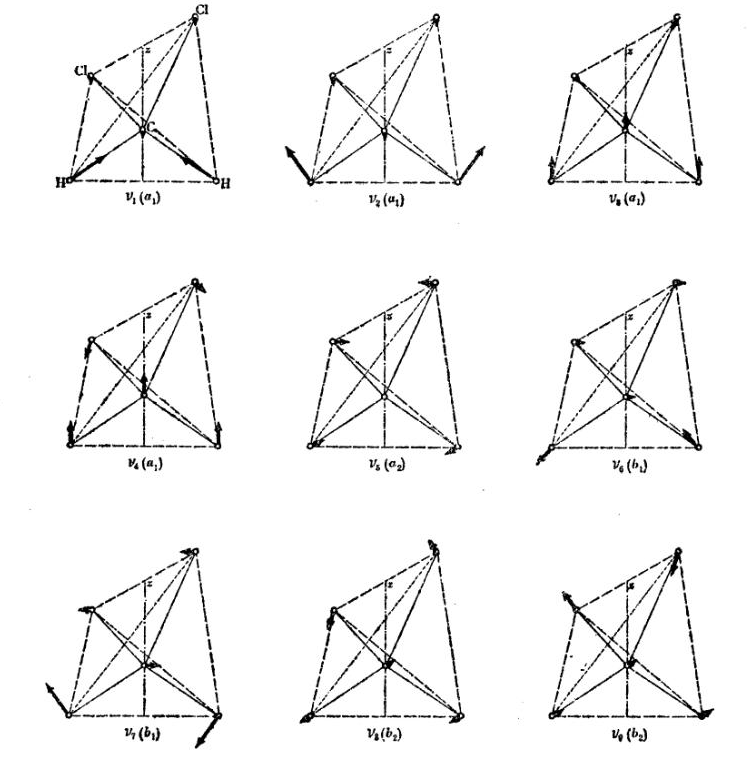
\includegraphics[width=0.8\textwidth]{figures/ch2cl2.png}
            \label{fig:ch2cl2-schwingungen}
          }
          \caption[Aufgezeichnete Spektren von $\mathrm{CH_2Cl_2}$ und mögliche Schwingungen des Moleküls.]{\protect\subref{fig:chcl3-ch2cl2} Aufgezeichnete Spektren von $\mathrm{CH_2Cl_2}$ im Vergleich mit $\mathrm{CHCL_3}$, jeweils mit Polarisationsfilter in Nullstellung. \protect\subref{fig:ch2cl2} Spektren von $\mathrm{CH_2Cl_2}$ mir Winkel des Polarisationsfilter $\theta=\ang{0},\ang{90}$. \protect\subref{fig:ch2cl2} Mögliche Schwingungen des $\mathrm{CH_2Cl_2}$-Moleküls. \cite{herzberg}}
          \label{fig:ch2cl2-analyse}
        \end{figure}


    \section{Kohlenstoffringe}

      \begin{figure}[tb]
        \subfloat[]{
          \chemfig{H-C*6(=C(-H)-C(-H)=C(-H)-C(-H)=C(-H)-)}
          \label{fig:c6h6-molecule}
        }
        \subfloat[]{
          \chemfig{C(-[::210]H)(-[::150]H)*6(-C(-[::-90]H)(-[::-30]H)-C(-[::-90]H)(-[::-30]H)-C(-[::-90]H)(-[::-30]H)-C(-[::-90]H)(-[::-30]H)-C(-[::-90]H)(-[::-30]H)-)}
          \label{fig:c6h12-molecule}
        }
        \subfloat[]{
          \chemfig{N(=[::210]O)(-[::150]O)-C*6(=C(-H)-C(-H)=C(-H)-C(-H)=C(-H)-)}
          \label{fig:c6h5no2-molecule}
        }
        \caption[Molekülstrukturen der untersuchten Kohlenstoffringe.]{Molekülstrukturen der untersuchten Kohlenstoffringe. \protect\subref{fig:c6h6-molecule} Benzolring ($\mathrm{C_6H_6}$) \protect\subref{fig:c6h12} Cyclohexan ($\mathrm{C_6H_{12}}$) \protect\subref{fig:c6h5no2-molecule} Nitrobenzol ($\mathrm{C_6H_5NO_2}$)}
        \label{fig:kohlenstoffringe-molekuele}
      \end{figure}

      Die Molekülstrukturen der untersuchten Kohlenstoffringe Benzol ($\mathrm{C_6H_6}$), Cyclohexan ($\mathrm{C_6H_{12}}$) und Nitrobenzol ($\mathrm{C_6H_5NO_2}$) sind in \cref{fig:kohlenstoffringe-molekuele} dargestellt. Der bei jedem der Moleküle auftretenden innere Kohlenstoffring lässt eine starke Raman-Linie bei entsprechend der C-C-Streckschwingung bei $\SI{1206}{\per\centi\meter}$ (vgl. \cref{subsec:harm-oszi-absch}) erwarten. Weiter enthalten alle Moleküle mindestens fünf C-H-Bindungen, sodass außerdem deren Streckschwingung als Maximum in den Spektren bei $\SI{3063}{per\centi\meter}$ (vgl. \cref{subsec:harm-oszi-absch}) zu erwarten ist.

      Die aufgenommenen Spektren sind in \cref{fig:ringe} abgebildet. Sowohl für $\mathrm{C_6H_6}$, als auch für $\mathrm{C_6H_5NO_2}$ sind die die Raman-Linie der C-H-Streckschwingung an erwarteter Stelle zu finden. Lediglich beim $\mathrm{C_6H_{12}}$-Molekül treten anstelle der einzelnen Linie zwei, zu etwas kleineren Raman-Verschiebungen verschobene Maxima auf. Diese können als die beiden Streckschwingungen der $\mathrm{CH_2}$-Moleküle identifiziert werden.

      Da die C-H-Streckschwingung symmetrisch ist, muss das Maximum stark polarisiert sein. Enstprechend werden die Maxima des Benzolrings bei $\sim\SI{994}{\per\centi\meter}$, des Cyclohexanrings bei $\sim\SI{801}{\per\centi\meter}$ und des Nitrobenzolrings bei $\sim\SI{1003}{\per\centi\meter}$ dieser Schwingung zugeordnet. Bei letzter ist nicht auszuschließen, dass einer der anderen Maxima in diesem Bereich der Raman-Verschiebung der Richtige ist, da alle größteteils polarisiert sind. Jedoch ist die Molekularstruktur derer von Benzol so ähnlich, dass eine äquivalente Raman-Verschiebung zu erwarten ist. Die zugeordnete Streckschwingung wird als Streckung des Rings bezeichnet, da bei gleichphasigem Schwingen der C-C-Bindungen der Durchmesser des Rings ändert.

      \begin{figure}[tb]
        \centering
        \subfloat[]{
        \tikzsetnextfilename{C6H6}
          \begin{tikzpicture}
            \begin{axis}[
              /tikz/line join=bevel,
              width=0.45*\textwidth,
              height=0.45*\textwidth,
              grid,
              legend style={at={(1,1)}, legend columns=1, anchor=north east},
              every axis plot,
              xmin = 0, xmax = 3500,
              %ymin = \Pmin, ymax = \Pmax,
              xlabel = {Raman-Verschiebung $\Delta \nu$ in $\si{\per\centi\meter}$},
              ylabel = {Zählrate $n$},
              %xtick = {0,500, 1000, ..., 3500},
              /pgf/number format/use comma,
              /pgf/number format/1000 sep={},
              ]
              % Add plots
              %\addplot[color=red,  line width = 0.5pt] table [x=raman,y=n]{data/CCl4_pol0.txt};
              %\addlegendentry{$\mathrm{CCl_4}$}
              \addplot[color=red,  line width = 0.5pt] table [x=raman,y=n]{data/C6H6_pol0.txt};
              \addlegendentry{$\theta_\mathrm{pol}=\ang{0}$}
              \addplot[color=blue,  line width = 0.5pt] table [x=raman,y=n]{data/C6H6_pol1.txt};
              \addlegendentry{$\theta_\mathrm{pol}=\ang{90}$}
            \end{axis}
          \end{tikzpicture}
          \label{fig:c6h6}
        }
        \subfloat[]{
        \tikzsetnextfilename{C6H12}
          \begin{tikzpicture}
            \begin{axis}[
              /tikz/line join=bevel,
              width=0.45*\textwidth,
              height=0.45*\textwidth,
              grid,
              legend style={at={(1,1)}, legend columns=1, anchor=north east},
              every axis plot,
              xmin = 0, xmax = 3500,
              %ymin = \Pmin, ymax = \Pmax,
              xlabel = {Raman-Verschiebung $\Delta \nu$ in $\si{\per\centi\meter}$},
              ylabel = {Zählrate $n$},
              %xtick = {0,500, 1000, ..., 3500},
              /pgf/number format/use comma,
              /pgf/number format/1000 sep={},
              ]
              % Add plots
              \addplot[color=red,  line width = 0.5pt] table [x=raman,y=n]{data/C6H12_pol0.txt};
              \addlegendentry{$\theta_\mathrm{pol}=\ang{0}$}
              \addplot[color=blue,  line width = 0.5pt] table [x=raman,y=n]{data/C6H12_pol1.txt};
              \addlegendentry{$\theta_\mathrm{pol}=\ang{90}$}
            \end{axis}
          \end{tikzpicture}
          \label{fig:c6h12}
        } \\
        \subfloat[]{
        \tikzsetnextfilename{C6H5NO2}
          \begin{tikzpicture}
            \begin{axis}[
              /tikz/line join=bevel,
              width=0.45*\textwidth,
              height=0.45*\textwidth,
              grid,
              legend style={at={(1,1)}, legend columns=1, anchor=north east},
              every axis plot,
              xmin = 0, xmax = 3500,
              %ymin = \Pmin, ymax = \Pmax,
              xlabel = {Raman-Verschiebung $\Delta \nu$ in $\si{\per\centi\meter}$},
              ylabel = {Zählrate $n$},
              %xtick = {0,500, 1000, ..., 3500},
              /pgf/number format/use comma,
              /pgf/number format/1000 sep={},
              ]
              % Add plots
              \addplot[color=red,  line width = 0.5pt] table [x=raman,y=n]{data/C6H5NO2_pol0.txt};
              \addlegendentry{$\theta_\mathrm{pol}=\ang{0}$}
              \addplot[color=blue,  line width = 0.5pt] table [x=raman,y=n]{data/C6H5NO2_pol1.txt};
              \addlegendentry{$\theta_\mathrm{pol}=\ang{90}$}
            \end{axis}
          \end{tikzpicture}
          \label{fig:c6h5no2}
        }
        \caption[Spektren der Kohlenstoffwasserstoff-Ringe und exemplarische Struktur eines Benzolrings.]{Spektren der Kohlenstoffwasserstoff-Ringe \protect\subref{fig:c6h6} $\mathrm{C_6H_6}$, \protect\subref{fig:c6h12} $\mathrm{C_6H_{12}}$, \protect\subref{fig:c6h5no2} $\mathrm{C_6H_5NO_2}$. }
        \label{fig:ringe}
      \end{figure}

      \Cref{fig:ringe} zeigt die Spektrend er zyklischen Kohlenstoffwasserstoff-Ringe Benzol ($\mathrm{C_6H_6}$), Cyclohexan ($\mathrm{C_6H_{12}}$) und Nitrobenzol ($\mathrm{C_6H_5NO_2}$).


  \section{Temperaturbestimmung von kristallinem Schwefel}

    Durch das Verhältnis der Zählraten von Stokes- und Anti-Stokes-Maximum der prominenten Eigenschwingung von Schwefel soll hier die Temperatur des kristallinen Schwefels bestimmt werden. Dazu werden die Maxima bei $\sim\pm\SI{470}{\per\centi\meter}$ des in \cref{fig:schwefel} betrachtet. Aufgrund der Breite der Maxima und des Umstandes, dass das Rayleigh-Maximum nicht genau auf $\nu=\SI{0}{\per\centi\meter}$ liegt, wird ein Fehler von
    \begin{equation*}
      \delta \nu = \pm\SI{10}{\per\centi\meter}
    \end{equation*}
    angenommen.

    Umformen von gleichung \cref{eq:stokesvergleich} nach der Temperatur $T$ ergibt unter Verwendung von
    \begin{equation*}
      \omega_n = 2\pi c \Delta \nu_\mathrm{Stokes}
    \end{equation*}
    und der Kreisfrequenz der Laserstrahlung
    \begin{equation*}
      \omega = \frac{2\pi c}{\lambda_\mathrm{L}},
    \end{equation*}
    mit $\lambda_\mathrm{L}=\SI{532}{\nano\meter}$, gerade
    \begin{equation*}
      T = \frac{h \Delta \nu  c}{k_\mathrm{B}\ln\left[ \frac{n_\mathrm{Stokes}}{n_\mathrm{Anti-Stokes}} \left( \frac{\frac{1}{\lambda_\mathrm{L}} - \Delta \nu_\mathrm{Stokes}}{\frac{1}{\lambda_\mathrm{L}}+\Delta \nu_\mathrm{Stokes}} \right)^4 \right]}=\SI{19}{\celsius},
    \end{equation*}
    wobei $n_\mathrm{Stokes},n_\mathrm{Anti-Stokes}$ die entsprechenden Zählraten von Stokes- und Anti-Stokes-Maximum sind. Weiter bezeichnet $h$ das Plancksche Wirkungsquantum, $k_\mathrm{B}$ die Boltzmann-Konstante.

    \begin{figure}
      \centering
      \tikzsetnextfilename{schwefel}
      \begin{tikzpicture}
        \begin{axis}[
          /tikz/line join=bevel,
          width=0.8*\textwidth,
          height=0.5*\textwidth,
          grid,
          legend style={at={(1,1)}, legend columns=1, anchor=north east},
          every axis plot,
          xmin = -600, xmax = 600,
          %ymin = \Pmin, ymax = \Pmax,
          xlabel = {Raman-Verschiebung $\Delta \nu$ in $\si{\per\centi\meter}$},
          ylabel = {Zählrate $n$},
          %xtick = {0,500, 1000, ..., 3000},
          /pgf/number format/use comma,
          /pgf/number format/1000 sep={},
          ]
          % Add plots
          \addplot[color=red,  line width = 0.5pt] table [x=raman,y=n]{data/Schwefel_pol0.txt};
          \addlegendentry{$\theta_\mathrm{pol}=\ang{0}$}
        \end{axis}
      \end{tikzpicture}
      \caption[Spektrum von kristallinem Schwefel.]{Spektrum von kristallinem Schwefel. Wichtig für die Auswertung sind die Zählraten der prominenten Stokes- und Anti-Stokes-Maxima.}
      \label{fig:schwefel}
    \end{figure}











\end{document}
